\documentclass[10pt, conference]{IEEEtran}

% correct bad hyphenation here
%\hyphenation{op-tical net-works semi-conduc-tor}

\usepackage{url}
\usepackage{graphicx}
\usepackage{dcolumn}
\usepackage{color}

\newcommand{\nPrograms}{250,163}
\newcommand{\nAnalyzedPrograms}{247,798}
\newcommand{\nemptyPrograms}{14,307}
\newcommand{\nScriptPrograms}{233,491}
\newcommand{\nLOC}{36,085,654}
\newcommand{\nscripts}{4,049,356}


\newcommand{\fenia}[1]{\emph{\color{blue}Fenia says: #1}}
\newcommand{\felienne}[1]{\emph{\color{green}Felienne says: #1}}
\newcommand{\grex}[1]{\emph{\color{yellow}Gregorio says: #1}}
\newcommand{\jemole}[1]{\emph{\color{red}Jesús says: #1}}

\begin{document}

\title{A dataset of Scratch programs,\\Scraped, Shaped and Scored}


\author{
	\IEEEauthorblockN{Efthimia Aivaloglou\IEEEauthorrefmark{1}, Felienne Hermans\IEEEauthorrefmark{1}, Gregorio Robles\IEEEauthorrefmark{2}, and Jes{\'u}s Moreno-Le{\'o}n\IEEEauthorrefmark{3}}
	
	\IEEEauthorblockA{\IEEEauthorrefmark{1}Delft University of Technology, The Netherlands\\
			Email: \{e.aivaloglou, f.f.j.hermans\}@tudelft.nl}
	\IEEEauthorblockA{\IEEEauthorrefmark{2}Universidad Rey Juan Carlos, Fuenlabrada (Madrid), Spain \\
		Email: grex@gsyc.urjc.es}
	\IEEEauthorblockA{\IEEEauthorrefmark{3}Programamos.es \& Universidad Rey Juan Carlos, Spain\\
		Email: jesus.moreno@programamos.es}
}

\maketitle


\begin{abstract}
In this paper, we present a collection of 250K Scratch programs scraped from the Scratch project repository. We processed the program data to encode it into a database that facilitates querying and further analysis. The dataset is intended as an input for research on computing education and source code analysis.
\end{abstract}

\begin{IEEEkeywords}
Scratch; dataset;
\end{IEEEkeywords}


 
\section{Introduction}
Scratch \cite{resnick_scratch:_2009} is a block-based programming language developed to serve as a stepping stone for children from 8 to 16 years old to the more advanced world of computer programming.
It offers a web-based programing environment that enables creating games and interactive animations. The public repository of Scratch programs contains over 19 million projects and 16 million users.

A number of works in the computing education research field attempt to assess the programming skills that novice programmers develop in the Scratch environment.
Some utilize program data collected during specific programming courses (e.g., \cite{meerbaum-salant_learning_2010, wilson_evaluation_2012, Maloney_2008}), while others utilize the dataset made available by the Lifelong Kindergarten Group at the MIT Media Lab, which contains data for Scratch projects created until 2012 (e.g., \cite{fields_2014, yang_2015, Dasgupta_2016}).
In addition to identifying indications of learning of programming concepts, static analysis of Scratch programs has also been performed for identifying code smells and bad programming practices within Scratch programs \cite{Meerbaum_habits_2011, Aivaloglou_2016}, and automated quality assessment tools have been proposed (e.g. Hairball \cite{boe_hairball:_2013} and Dr. Scratch \cite{moreno_automatic_2014}).

While Scratch is receiving increasing interest as an introductory programming language, there is no recent dataset of Scratch programs available to the research community.
The one made available from the MIT Media Lab concerns projects created using the previous, initial version of the Scratch application, before the introduction of the Scratch 2 web programming interface in 2013.
It is since then that the popularity of Scratch started increasing\footnote{Monthly activity trends can be found at \url{https://scratch.mit.edu/statistics/}}.

The goal of this paper is to present an open and timely dataset of recent Scratch programs, along with their metadata, that can facilitate quantitative research in the fields of source code analysis and computing education.
The dataset contains 250 thousand Scratch projects, from more than 100 thousand different users, that were scraped from the Scratch project repository.
It is made available as a database\footnote{{\fenia{add anonymized address, update it in repo footnote}}} which includes, for each Scratch project, its metadata and the program data, along with programming mastery scoring results from the Dr. Scratch quality assessment tool \cite{moreno_automatic_2014}.

\section{Dataset Construction}
\label{dataset}

\subsection{Data collection}
To collect the data from the web interface of the Scratch project repository we built a scraping program.
The web scraping program, called Kragle, starts by reading the Scratch projects page\footnote{\label{scratchpublic}\url{https://scratch.mit.edu/explore/projects/all/}} and thus obtains the project identifiers of projects that were most recently shared.
Subsequently, Kragle retrieves the JSON code for each of the listed projects\footnote{For a given project id $x$, the program's JSON representation can be obtained via \url{https://cdn.projects.scratch.mit.edu/internalapi/project/x/get}}.

We ran Kragle on March 2nd 2016 for 24 hours and, during that time, it obtained the JSON code for \nPrograms projects. Out of those, we failed to parse and further analyze 2,367 projects due to technical difficulties with the JSON files.
Kragle, as well as all scraped projects and our analysis files are available.\footnote{\label{repo}\url{https://github.com/TUDelftScratchLab/ScratchDataset}}

Once we obtained the Scratch projects, we parsed the JSON files according to the specification of the format\footnote{\url{http://wiki.scratch.mit.edu/wiki/Scratch_File_Format_(2.0)}}.
This resulted in a list of used blocks per project, within the sprites and the stage of the project.
We also cross referenced all blocks with the Scratch wiki to determine the shapes and the category of all blocks.
For example, \texttt{When Green Flag Clicked} is a \emph{Hat block} from the \emph{Events category}.
We included the blocks from Scratch extensions, such as the LEGO WeDo extensions, that we found in the dataset.

\subsection{Calculation of programming mastery scores}
\fenia{Description of how the mastery metrics for       
	[Abstraction]
	,[Parallelism]
	,[Logic]
	,[Synchronization]
	,[FlowControl]
	,[UserInteractivity]
	,[DataRepresentation]
	,[Mastery]
	,[Clones]
	,[CustomBlocks]
	,[InstancesSprites]
	were calculated}

\subsection{Importing the data}
\label{dataAnalysis}
All scraped project data and metadata, including the list of used blocks and parameters, were imported in a relational database.
We also imported the data on the shapes and the categories of the Scratch blocks.
We then used SQL queries for normalizing the data and bringing it in its final schema, outlined in Table \ref{tbl-dbschema}.

\begin{table}[]
	\centering
	\begin{tabular}{llp{5.4cm}}
		\textbf{Table}& \textbf{Key} & \textbf{Attribute(Description)}\\
		\hline
		\textbf{\texttt{project}} & PK & \texttt{p\_id} (Scratch project ID)\\
		&  & 							\texttt{project-name} (name given to project)\\
		&  & 							\texttt{username} (author's Scratch 
		username)\\
		&  & 							\texttt{total-views} (project views number)\\
		&  & 							\texttt{total-remixes} (project remixes number)\\
		&  & 							\texttt{total-favorites} (total users favoriting)\\
		&  & 							\texttt{total-loves} (total users `loving' the project)\\
		& & 							\texttt{is-remix} (calculated column, true if project is a remix of another one)\\
		\hline
		\textbf{\texttt{script}} & PK & \texttt{script\_id} (auto increment)\\
		& FK & 							\texttt{project\_id} (\texttt{\scriptsize{*\ldots1 project:p\_id}})\\
		& & 							\texttt{sprite-type} (one of [sprite, stage, procDef])\\
		& & 							\texttt{sprite-name} (name sprite the script is in)\\
		& & 							\texttt{script-rank} (project-level ranking of script)\\
		& & 							\texttt{coordinates} (x-y location of script in Scratch editor)\\
		& & 							\texttt{total-blocks} (calculated column, number of blocks comprising the script)\\
		\hline
		\textbf{\texttt{procedure}} & PK,FK & \texttt{script\_id} (\texttt{\scriptsize{1\ldots1 script:script\_id}})\\
		& & 							\texttt{proc-name} (name given to custom block)\\
		& & 							\texttt{total-args} (number of input arguments)\\
		\hline
		\textbf{\texttt{block}} & PK,FK  & \texttt{script\_id} (\texttt{\scriptsize{*\ldots1 script:script\_id}})\\
		& PK & \texttt{block-rank} (script-level ranking of block)\\
		& FK & \texttt{block-type} (\texttt{\scriptsize{*\ldots1 blockType:b-type}})\\
		&  & \texttt{parameter-1} (value of 1st input parameter)\\
		&  &\vdots\\
		&  & \texttt{parameter-24} (value of 24th input parameter)\\
		\hline
		\textbf{\texttt{blockType}} & PK & \texttt{b-type} (Scratch name of predefined block)\\
		&  & \texttt{category} (Scratch block category)\\
		&  & \texttt{shape} (One of the 8 block shapes in the Scratch interface)\\
		&  & \texttt{is-input} (true if the block receives user input)\\
		\hline
		\textbf{\texttt{remix}} & PK  & \texttt{remix\_id} (\texttt{\scriptsize{project\_id}} of created project)\\
		&  & \texttt{from-project\_id} (\texttt{\scriptsize{project\_id}} of original project)\\
		\hline
		\textbf{\texttt{grades}} & PK,FK & \texttt{project\_id} (\texttt{\scriptsize{1\ldots1 project:p\_id}})\\
		& & \texttt{Abstraction} (\fenia{short descriptions})\\
		& & \texttt{Parallelism} ()\\
		& & \texttt{Logic} ()\\
		& & \texttt{Synchronization} ()\\
		& & \texttt{FlowControl} ()\\
		& & \texttt{UserInteractivity} ()\\
		& & \texttt{DataRepresentation} ()\\
		& & \texttt{Mastery} ()\\
		& & \texttt{Clones} ()\\
		& & \texttt{CustomBlocks} ()\\
		& & \texttt{InstancesSprites} ()\\
		\hline
	\end{tabular}
	\caption{Database schema: Tables and Attributes}
	\label{tbl-dbschema}
\end{table}

\section{Dataset Description}

\subsection{Data Representation}

The projects' data are stored in a relational database. Each \textbf{\texttt{project}} is identified by its Scratch project ID, stored in field \texttt{p\_id}, while its author is identified by the \texttt{username}\footnote{\label{fn-authorpage}Each project and author page can be accessed in the Scratch web interface at \url{https://scratch.mit.edu/projects/<p_id>} and \url{https://scratch.mit.edu/users/<username>} respectively}.
If a project is a remix of another one, the original project can be found in the \textbf{\texttt{remix}} table.
Table \textbf{\texttt{grades}} stores the Dr. Scratch results for the programming mastery metrics per project.
 
 \begin{figure}
 	\centering
 	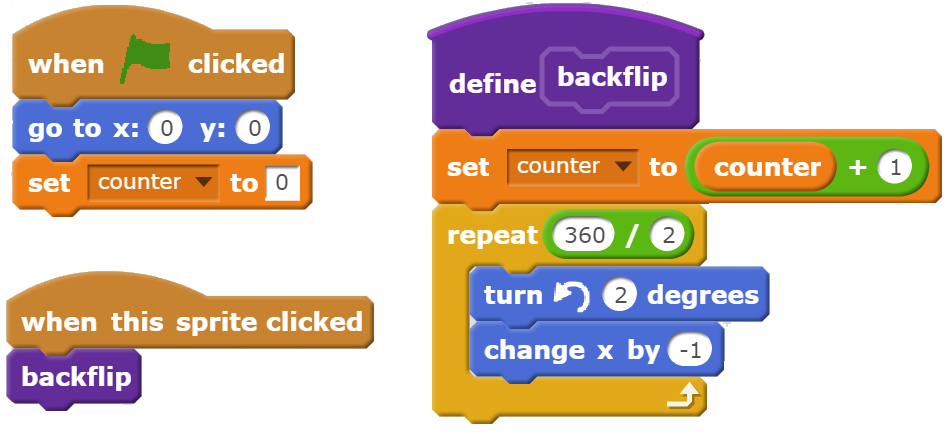
\includegraphics[width=0.45\textwidth]{scratchExample}
 	\caption{Example of a Scratch program with three scripts in the same spite}
 	\label{fig-scratchExample}
 \end{figure}

The schema of the database, outlined in Table \ref{tbl-dbschema}, reflects the structure of the Scratch programs.
Projects contain sprites, which are entities with their own associated code.
The code is organized into \textbf{\texttt{script}}s, i.e., groups of Scratch code blocks, each script belonging a sprite named \texttt{sprite-name}.
In the example in Figure \ref{fig-scratchExample} there are 3 scripts, one initiated when the green flag is clicked, one then the sprite is clicked, and the `backflip' custom block definition.
Those custom blocks are the equivalent of procedure definitions, with their names and arguments stored in the \textbf{\texttt{procedure}} table.

The coding elements in the Scratch environment are the \textbf{\texttt{block}}s, which can receive input parameters.
In the example in the figure, block `go to x:0 y:0' receives as input two numerical parameters.
Custom clock invocations are stored in this table just like regular blocks.
To cater for the varying number of input parameters that those blocks can have, this table can store up to the maximum number of input parameters found in the dataset, which is 24.
The ordering of the blocks in the scripts can be retrieved using the \texttt{block-rank} field, which represents a depth-first ranking of the blocks.
In the script of the `backflip' custom block definition in the example, the ranking of the blocks would be `define backflip', `set counter to', `+', `counter', followed by the rest of the blocks.
The clocks can be of different shapes and categories.
In table \textbf{\texttt{blockType}} we have stored the encoding of all types of Scratch blocks and the blocks from Scratch extensions.

\subsection{Dataset Contents}

\begin{table*}[]
	\centering
	\begin{tabular}{lrrrrrr}
		&\textbf{mean}&\textbf{min}&\textbf{Q1}&\textbf{median}&\textbf{Q3}&\textbf{max}\\
		\hline
		Projects per username&2.27&1&1&1&2&868\\
		Sprites per project&5.30&0&1&2&5&525\\
		Scripts per project&16.19&0&2&4&11&3,038\\
		Blocks per project&144.25&0&9&26&69&34,622\\
		Custom block definitions per project&0.64&0&0&0&0&372\\
		Total views per project&5.76&0&1&1&4&27,993\\
		Total remixes per project&197.12&0&0&0&0&14,951,164\\
		Total favorites per project&0.54&0&0&0&0&2,582\\
		Dr. Scratch mastery score per project&8.92&0&6&8&11&21\\
		\hline
	\end{tabular}
	\caption{Summary statistics of the dataset}
	\label{tbl-stats}
\end{table*}

\begin{table}[]
	\centering
	\begin{tabular}{lr}
		\hline
		Projects & 250,163 \\
		Non-empty projects & 233,491 \\
		Remixes of other projects & 12,167 \\
		Usernames & 109,960 \\
		Scripts & 4,049,356 \\
		Blocks & 36,085,654 \\
		Custom block definitions & 209,769 \\
		Projects analyzed by Dr. Scratch & 231,050 \\
		\hline
	\end{tabular}
	\caption{Dataset contents}
	\label{tbl-size}
\end{table}

As shown in Table \ref{tbl-size}, the dataset contains the metadata of 250,163 Scratch projects and the code of 233,491 of those that are non-empty.
The projects were created from 109,960 different users.
Most of those, as shown in Table \ref{tbl-stats}, have created a single project.
However, 40 thousand users have created more than one and up to 868 projects in the dataset.

The majority of the projects have been viewed only once, and they have not been favorited or remixed.
Around 10 thousand of the total projects have been remixed at least once, while the dataset includes cases of very popular projects with more than 100 remixes and even one thousand cases with more than 100 views. 

Table \ref{tbl-stats} also reveals the median project in the dataset: it contains 2 sprites, 4 scripts, 26 blocks, no custom block definitions, and receives a mastery score of 8 our of 21.
The table also highlights the existence of surprisingly complex projects, with 525 sprites, 3 thousand scripts as 34 thousand blocks.

\fenia{Should we add some stats about the Dr Scratch master scores?}

\section{Enabled Research and Dataset Extension}
\fenia{What about our own papers utilizing the dataset? (\cite{Aivaloglou_2016} and \cite{Robles_2017}). We have to anonymize the submission, so do we add them now or add a note that we omitted them and add them to the camera ready?}

The evaluation of block-based languages in general, and Scratch in particular, as tools for programming education is receiving significant research attention.
A number of studies have been carried out during the last years on understanding of programming concepts and the programming practices of novice programmers in block-based environments, on the programming skills they develop, and on the quality of Scratch programs.

The first research direction that this dataset can be utilized for concerns the \textit{assessment of the programming skills that novice programmers develop in the Scratch environment}.
The dataset can be used for examining indications of learning of programming concepts and abstractions.
Existing works in this research direction include the work by Maloney \emph{et al.} \cite{Maloney_2008}, who analyzed 536 Scratch projects created in an after-school clubhouse for blocks that relate to programming concepts including loops, conditional statements, variables, user interaction, synchronization, and random numbers, and found that within the least utilized ones are boolean operators and variables.
Another study on the internalization of programming concepts with Scratch with 46 students was presented in \cite{meerbaum-salant_learning_2010}.
Concepts like loops, conditional loops, message passing, initialization, variables and concurency were examined, and it was found that students had problems with the last three. In \cite{wilson_evaluation_2012}, 29 projects created by 60 students working in groups were evaluated based on a list of criteria related to programming concepts, code organization and usability design.

Towards this research direction, the dataset makes the source code of the Scratch programs available for static analysis and can be used for quantitatively evaluating the application of programming concepts and abstractions through the presence of Scratch blocks of the corresponding types.

Another promising research direction relates to the \textit{quality of the programming artifacts developed in the Scratch environment}.
The dataset can be used for quality assessment, for the identification of programming smells, and for exploring indications of harmful programming habits.
Existing works in this direction include a study in a classroom setting \cite{Meerbaum_habits_2011}, which highlighted two bad programming habits in Scratch, namely bottom-up development and extremely fine-grained programming.
The authors connected the later to the reduced use of if-blocks and finite loops and the increased use of infinite loops.
Related to smell detection are the Scratch automated quality analysis tools Hairball \cite{boe_hairball:_2013}, a lint-like static analysis tool for Scratch that can detect initialization problems and unmatched broadcast and receive blocks, and Dr. Scratch \cite{moreno-leon_dr._2015}, which extends Hairball to detect two bad programming habits in Scratch: not changing the default object names and duplicating scripts.

This dataset will enable examining code quality and code smells on a large set of Scratch projects.
Static analysis of the source code can also be performed for the identification of other types of smells \cite{fowler_refactoring:_1999} that might be common in the artifacts of novice programmers.

Moving from the software engineering to the computing education research field, a research direction with increased data requirements concerns the \textit{learning progressions of novice programmers}.
This includes examining the factors that support learning and improving their programming skills.
Existing works in this area have used the dataset of Scratch programs created until 2012, before the current web-based programming environment was introduced, and described in the Introduction.
They include the works of Dasgupta et al., who investigated how project remixing relates to the adoption of new computational thinking concepts \cite{Dasgupta_2016}, and Yang et al., who examined the learning patterns of programmers in terms of block use over their first 50 projects \cite{yang_2015}.

Enabling research towards this direction requires extending the dataset with the complete set of projects for the included users, along with their creation dates.
This would enable examining how the programming skills and mastery of the users evolved through time, possibly through remixing the projects of other users.
An even richer extension of the dataset would be with, possibly daily, snapshots of the included projects that are still in development.
This would enable reconstructing some project versioning information, not available from the Scratch web interface, and thus examining how the projects are developed and evolve over time.

Apart from quantitative studies, the dataset can support the design of experiments and field studies, whose material often includes Scratch programs with specific characteristics.
For example, in \cite{hermans_2016} examples of Scratch programs exhibiting specific smells were used in a controlled experiment to determine how the smells affected the understanding and the modification of the programs.
This queryable dataset can support finding example programs with characteristics according to the experiment design and the field of the study.

\section{Limitations}
The only information about the authors of the Scratch projects contained in the dataset is their username.
This suffices for creating project portfolios of the authors and facilitating research in the directions described in the previous section.
However, other directions in the computing education research field require richer author data, and especially data on their gender and their age.
There are, for example, indications that specific programming concepts are better understood after certain ages ---Seiter and Foreman \cite{Seiter_2013} analyzed 150 Scratch projects from primary school students and found that design patterns requiring the understanding of parallelization, conditionals and, especially, variables were under-represented by all grades apart from 5 an 6.
The effect of gender and account age were also examined in \cite{fields_2014} in relation to the use of programming concepts.
Studies on the effect of parameters like the age are not only interesting but also of direct value to educators, since they give insights on when it is better to introduce computational thinking concepts in the curriculum of schools.
However, this dataset does not include information on the gender and the age of authors and cannot be extended to do so using the current Scratch web interface because this information is not available in the user profile page\footnotemark[\ref{fn-authorpage}], even though it is provided by the users upon registration.

Another limitation of this dataset is that we did not scrape a random sample of Scratch projects, but the 250,000 most recent ones during the time that we run the scraper.
It could be the case that the programming habits of Scratch users are changing over time.
However, we counterbalanced that by collecting a large dataset which comprises around 1.3\% of all 19 million shared Scratch projects, and is still the most recent one to be made available to the research community.

\section{Conclusion}
The increasing popularity of Scratch as an introductory programming language makes it an increasingly popular research target in the computing education research field.
This paper presented an open and timely dataset of recent Scratch programs, that can facilitate research in the fields of source code analysis and computing education.
The dataset can support various research topics, including the ones related to the assessment of the programming skills that novice programmers develop in the Scratch environment and the exploration of their learning progressions, and issues related to the quality of the programs and the identification of smells and bad programming habits.

The dataset contains 250 thousand Scratch projects, from more than 100 thousand different users, that were scraped from the Scratch project repository.
It is made available as a database\footnote{{\fenia{add anonymized address, update it in repo footnote}}} which includes the source code of the Scratch projects, their metadata, and their programming mastery scoring results.

\bibliographystyle{IEEEtran}
\bibliography{IEEEabrv,ScratchDataset}

\end{document}


